\chapter{انواع روش‌های طبقه‌بندی ترافیک شبکه}

از گذشته روش‌های مختلفی برای طبقه‌بندی ترافیک شبکه اینترنت وجود داشته‌است که در این بخش هر یک از این تکنیک‌ها را بررسی می کنیم. 

\section{روش مبتنی بر درگاه }
شناخته شده ترین و قدیمی ترین روش مورد استفاده برای طبقه بندی ترافیک اینترنت، تطبیق شماره ی درگاه است. در این روش، از شماره‌ی درگاه مقصد در سرآیند لایه انتقال
بسته برای شناسایی ترافیک استفاده می‌شود و مقدار شماره‌ی درگاه با لیست شماره درگاه های تعیین شده در استاندارد \lr{IANA}، برای شناسایی بسته جاری مقایسه می‌شود. در جدول 1 شماره درگاه اختصاص داده شده برای بعضی از برنامه‌های معروف آورده شده‌است. مثلا برنامه‌های وب از پورت 80 استفاده می‌کنند. \cite{iana}

\begin{table}[!h]
\caption{شماره درگاه‌های اختصاص داده شده به برخی از برنامه‌های پرکاربرد}
\centerline{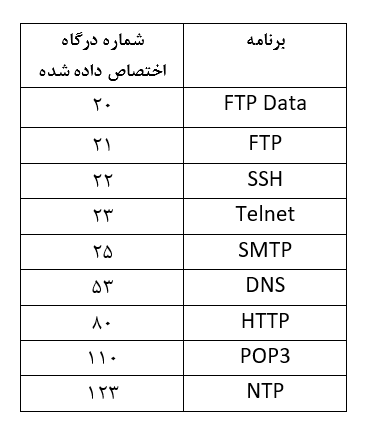
\includegraphics[width=0.5\textwidth]{ports.PNG}}
\end{table}

اما امروزه برنامه‌های جدید بخصوص برنامه‌های نظیر به نظیر از روش‌های مختلف برای پنهان کردن خود استفاده می‌کنند. آنها از درگاه‌های پویا و یا درگاه‌های دیگر برنامه‌های
شناخته‌شده در اتصالاتشان استفاده می‌کنند. که این امر باعث کاهش دقت طبقه‌بندی این روش شده‌است.

\section{روش مبتنی پیلود  }
با بوجود آمدن برنامه های نظیر به نظیر این روش، جایگزین قبلی شد. در این روش محتوای بسته‌ها برای پیدا کردن امضای برنامه‌های شناخته شده جستجو می‌شود. در جدول 2 یک نمونه از این امضاها که توسط کاراگیانیس\LTRfootnote{Thomas Karagiannis} استفاده شده است را می‌بینیم.

\begin{table}[!h]
\caption[نمونه امضاهای موجود در بسته های برخی از برنامه های پرکاربرد]{نمونه امضاهای موجود در بسته های برخی از برنامه های پرکاربرد\cite{shafiq2016network}}
\centerline{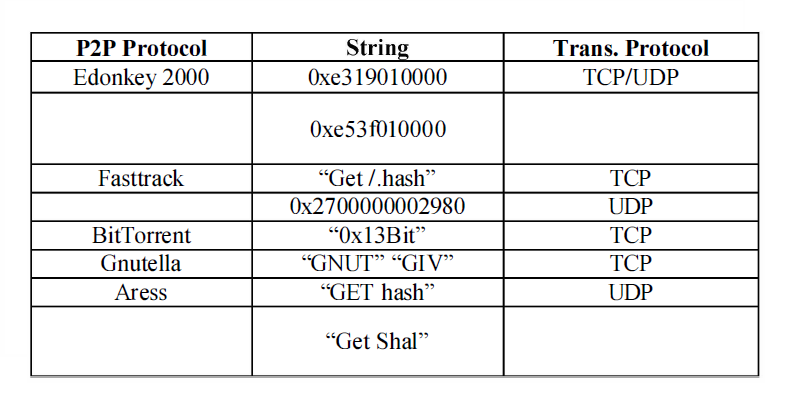
\includegraphics[width=0.9\textwidth]{signature.PNG}}
\end{table}

این روش به نسبت روش قبل دقیق تر عمل می‌کند اما چند مشکل دارد. مهم تر از همه این که نمی توان آن را بر روی بسته های رمزگذاری شده اعمال کرد. به علاوه تجزیه و تحلیل مستقیم داده ها باعث نقض حریم خصوصی کاربران می‌شود. همچنین این روش چون محتویات تمام بسته ها را بررسی میکند، نیازمند سیستم پردازشی به مراتب قوی تری نسبت به روش های دیگر است.

\section{روش مبتنی بر رفتار میزبان  }
ایده ی اصلی این روش این است که برنامه های مختلف الگوهای اتصال متفاوتی دارند. روش مبتنی بر رفتار میزبان، ارتباطات میان میزبان های خاص در یک شبکه را شناسایی میکند و الگوی ارتباط یک میزبان خاص با الگوی رفتار فعالیت های متفاوت مقایسه می‌شود. این روش پیلود بسته را برای طبقه بندی ترافیک استفاده نمی‌کند. پس می‌تواند بسته ها با محتوای رمزگذاری شده را نیز شناسایی کند.
\\
اما اشکال این روش این است که بیشتر تکنیک های مبتنی بر رفتار میزبان فرض می‌کند که میزبان های تحت نظارت در یک لحظه تنها از یک برنامه استفاده می‌کنند اما می‌دانیم در واقعیت، این وضعیت ممکن است هرگز اتفاق نیفتد. بیشتر کاربران از برنامه های زیادی به طور همزمان استفاده می‌کنند.
مشکل دیکری که در این روش بوجود میاد این است که برخی الگوهای رفتاری برنامه را نمی‌توان به آسانی کشف کرد. به مقدار حافظه و جریان های زیادی برای همه میزبان ها نیاز دارد تا بتواند الگوی اتصال را کشف کند. \cite{jangal}

\section{روش مبتنی بر یادگیری ماشین  }
یادگیری ماشین مجموعه ای از تکنیک‌ها برای داده کاوی و کشف دانش است که الگوهای ساختاری مفید در داده ها را جستجو میکند. این روش طبقه بندی مبتنی بر مجموعه داده های برچسب گذاری شده است. در این روش، یک طبقه بندی کننده یادگیری ماشین به عنوان ورودی آموزش داده می‌شود و سپس با استفاده از نمونه آموزش دیده، داده های ناشناخته طبقه بندی می‌شود.
دو روش اصلی در یادگیری ماشین وجود دارد. که در ادامه به بررسی هرکدام می‌پردازیم.

\subsection{یادگیری نظارت شده}
روش های یادگیری با نظارت، مبتنی بر دانش از پیش تعریف شده هستند. این الگوریتم ها در مرحله آموزش، نمونه های از پیش طبقه بندی شده (متشکل از ویژگی ها و
برچسب مرتبط با آنها) را به عنوان ورودی می‌گیرند و قوانین طبقه بندی ایجاد می‌شود. در مرحله طبقه بندی تلاش می‌کنند تا برچسب نمونه‌های بدون برچسب را پیشبینی
کنند.

\subsection{یادگیری بدون نظارت}
روش های یادگیری بدون نظارت، در مرحله یادگیری خود به هیچ دانش از قبل تعیین شده ای نیاز ندارند. این روش گروه های طبیعی را در داده ها کشف می‌کنند و روی کشف الگوهای موجود در داده ها تمرکز دارند. نمونه ها را بر اساس میزان شباهت ویژگی‌های آنها که توسط یک رویکرد اندازه گیری فاصله تعریف می‌شود. بنابر این در خروجی نمی‌توانیم نوع داده را به طور دقیق مشخص کنیم. صرفا داده های مشابه با هم در یک دسته قرار می‌گیرند.
\section{خلاصه}
در این فصل روش های کلی موجود برای طبقه بندی ترافیک شبکه از ابتدا تا کنون مورد بررسی قرار گرفت و راجع به مزایا و معیاب هر کدام بحث شد. روش مبتنی بر درگاه در برنامه های نظیر به نظیر دقت بالایی ندارد. روش مبتنی بر پیلود نیازمند سیستم پردازشی قوی می‌باشد و در شناسایی بسته های رمزگاری شده عاجز است. روش مبتنی بر رفتار میزبان صرفا برای زمان هایی که میزبان تنها از یک برنامه در لحظه استفاده می‌کند نتایج دقیقی تولید می‌کند. سپس روش های مبتنی بر یادگیری ماشین و انواع آن معرفی شد.
در ادامه روش مدل سازی و استفاده از یادگیری ماشین در طبقه بندی ترافیک شبکه توضیح داده می‌شود.. و سپس چند مورد از الگوریتم های معروف یادگیری ماشین و نیز پژوهش های انجام شده حول این موضوع بررسی می‌شود.